% Transformation #8 — Steric-Cliff Dethreading Schematic
% Figure 1 in the Transformation #8 Φ_c anchor subsection (SYNTHONICON.md / QUANTSYNTHONICON)
%
% SOURCE IMAGE: SYN_GROPPI.png (hand-drawn schematic, root directory)
%
% Axis convention:
%   y: free energy relative to dethreaded reference (negative = threading stabilisation)
%   x: dethreading coordinate — axle displacement, increasing right
%
% Quantitative values from: Groppi et al. Angew. Chem. Int. Ed. 2020, 59, 14825–14834
% DOI: 10.1002/anie.202003064
%
% This is a SCHEMATIC — not a reproduction of Groppi Fig. 7.
% Caption makes the distinction explicit.

\begin{figure}[htbp]
  \centering
  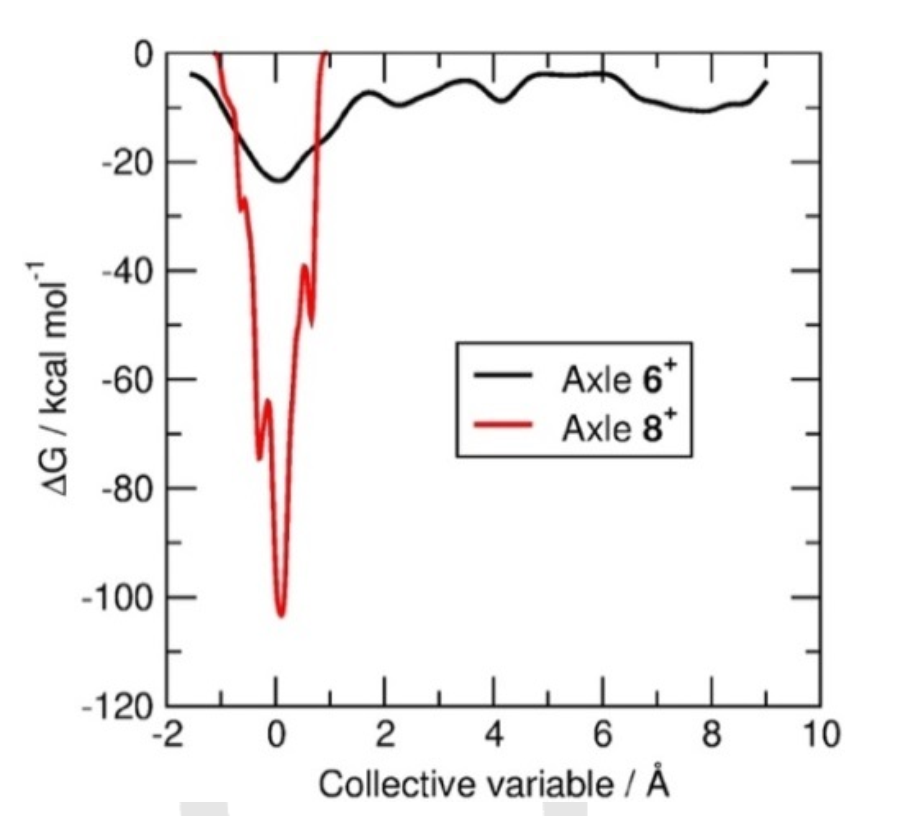
\includegraphics[width=0.60\textwidth]{SYN_GROPPI.png}
  \caption{
    \textit{Schematic} free-energy profiles for dethreading of DB24C8 with
    dialkylammonium guests (schematic representation; quantitative values from
    Groppi et al.\ \textit{Angew.\ Chem.\ Int.\ Ed.} \textbf{2020}, \textit{59},
    14825–14834, DOI: 10.1002/anie.202003064).
    %
    \textbf{Black curve} — guest \textbf{6}$^+$ (``good'' axle, on-axis methyl):
    descends into the threaded-complex minimum and exits via a moderate barrier
    $\Delta G^\ddagger \approx 19.8$ kcal mol$^{-1}$; ring-distortion modes
    $< 200$ cm$^{-1}$ remain thermally accessible ($K_\text{mod}$).
    %
    \textbf{Red curve} — guest \textbf{8}$^+$ (``bad'' axle, symmetric off-axis
    methyl): drops into a deep minimum with a near-discontinuous steric cliff;
    dethreading barrier $> 100$ kcal mol$^{-1}$; required ring-elongation modes
    at 614 and 809 cm$^{-1}$ lie far above $k_BT$ at 300~K (effective
    $K_\text{trap}$).
    %
    A sub-\AA{} methyl repositioning produces a $> 5\times$ barrier amplification
    with no change in the mechanical bond ($R_{\Leftrightarrow}$) or cyclic
    topology ($T_\bowtie$) — the all-or-nothing steric selectivity that yields
    provisional degeneracy\_strength $\approx 0.71$ (power-law/low-logarithmic
    boundary) and meets the $\Phi_c$ candidacy threshold of the Unified
    Synthonicon framework (Axiom~5).
  }
  \label{fig:groppi_schematic_t8}
\end{figure}
